% Idea 3 sections for the midterm report (draft). Paste into the team Overleaf.
% Needs in the preamble (if not already there): \usepackage{xcolor} \usepackage{amsmath,amssymb} \usepackage{booktabs}
% Placeholders for numbers that depend on the test run are marked \TBD{...}.
\providecommand{\TBD}[1]{\textcolor{red}{[#1]}}

% =====================================================================
% (A) Idea 3 pieces for the shared sections (hand these to whoever edits each section)
% =====================================================================

% --- Abstract: one sentence (finalize after the test run) ---
% Idea 3 asks whether a person's apparent trustworthiness, cued in text or by a face, sways a VLM's choice of socially
% appropriate action, and whether removing a trust direction estimated from language also removes the face's influence;
% \TBD{headline finding}.

% --- 1. Introduction: challenge paragraph (1 to 2 sentences) ---
% A socially competent model must react to what people do and visibly express, yet humans and language models also
% judge character from facial appearance \citep{lehr2026face}, an inference that is not valid evidence; because such
% impressions can reach a model through language or through vision, separating them from legitimate social signals is
% a multimodal problem.
% --- 1. Introduction: "In this paper" paragraph (1 sentence) ---
% Idea 3 measures how much an appearance-based trust cue moves Qwen3-VL's normative choices on EgoNormia and tests
% whether a trust direction estimated from text alone can be removed without erasing responses to behavior, and
% whether its removal transfers to faces.

% --- 2. Related Work: Idea 3 paragraph (trimmed for a shared 2/3 page) ---
\paragraph{Appearance-based trait inference and its removal.}
People infer trustworthiness from faces within a glance \citep{oosterhof2008functional}, and large language models reproduce this face-to-character mapping in consequential decisions \citep{lehr2026face}. Concepts in a model's residual stream are often carried by single directions that can be removed at inference time \citep{arditi2024refusal}, which \citet{ratzlaff2024debiasing} use to debias vision-language models; prompt-level rules offer a training-free alternative \citep{bai2022constitutional}. To our knowledge, no prior work tests whether appearance-based trust sways normative action choices in grounded egocentric scenes, or whether a trust direction estimated from language also governs a model's response to a face.

% --- 3. Problem Statement: notation request for its author (not text to paste) ---
% Idea 3 uses the shared x = (V, q, O), gold a^*, and the model distribution p_theta(o | x); it adds an optional context
% sentence c, written p_theta(o | x, c). If the shared statement can mention "an optional added context c", our notation
% plugs in directly. Idea 3's own objective is stated in Section 7.1.

% --- 4. Experimental Methodology: Idea 3 sentences ---
For Idea 3 we use the 1,184 EgoNormia items whose gold action is non-empty and whose options leave room for a trait cue, split by source video into train, validation and test (Section~7.1). As a second visual source we use One Million Impressions \citep{peterson2022omi}: 1,004 synthetic face images with mean human ratings of 34 attributes, including trustworthiness, happiness, age and gender, released under CC BY-NC-SA 4.0. We use the ratings only to select matched pairs of faces before any model is run.

% =====================================================================
% (B) Section 7 (data, splits and metrics are inside 7.1, as in Idea 1)
% =====================================================================
\section{Research Idea 3: Removing Appearance-Based Trust from Grounded Social Decisions}

\subsection{Initial Implementation}

\paragraph{Idea.}
When a vision-language model (VLM) chooses the appropriate next action in a real scene, the other person's \emph{apparent} trustworthiness should not matter: facial appearance is not valid evidence of character, even though humans and language models treat it as such \citep{oosterhof2008functional, lehr2026face}. What a person \emph{does} (holding a knife, returning a lost wallet) and the states they visibly express (anger, calm) are legitimate social signals. A useful fix must therefore remove the first influence while keeping the second. The same trust impression can reach a model through language (a sentence describing the person) or through vision (a face), which makes the problem multimodal: if both channels feed one internal representation, a correction estimated from text should also change how the model responds to faces. Our baseline tests this with activation steering on Qwen3-VL-8B-Instruct \citep{bai2025qwen3vl}.

\paragraph{Measurement.}
An item $x=(V,q,O)$ has five pre-action frames $V$, the question $q$ and $K=4$ candidate actions $O$ with gold action $a^\ast$. A cue $c$ is one sentence inserted before the question, for example ``The other person in the scene appears untrustworthy'' ($c_{\text{low}}$) or ``\dots appears trustworthy'' ($c_{\text{high}}$). We read the model's choice from its next-token distribution over the option letters,
\begin{align}
p_\theta(o_k \mid x,c)&=\operatorname{softmax}_k\, z_\theta(x,c)_{\ell_k},\\
\hat y(x,c)&=\textstyle\arg\max_k\, p_\theta(o_k\mid x,c),
\end{align}
where $z_\theta$ are the logits and $\ell_k$ is the token of the $k$-th letter; each item has one fixed random option order shared by every condition. Appearance sensitivity is the flip rate between matched low- and high-trust wordings,
\begin{equation}
S_{\text{app}}=\Pr\big[\hat y(x,c_{\text{low}})\neq\hat y(x,c_{\text{high}})\big],
\end{equation}
compared with the wording noise floor $S_0$ (a neutral sentence versus its paraphrase). Legitimate responsiveness $R_{\text{beh}}$ and $R_{\text{state}}$ are the analogous flip rates for negative versus positive behavior and expressed-state cues.

\paragraph{Data and evaluation.}
We use the EgoNormia items whose gold action is not the empty option and whose options leave room for a trait cue to matter (1,184 items, identified by the person-directed lexicon from our second assignment). We split by source video (50/15/35\%), giving 587 train, 196 validation and 401 test cue items; clean accuracy is computed on all items with a non-empty gold action in each split (921/289/622). Directions are estimated on train, the steering configuration is chosen on validation, and the test split is evaluated once after that choice is frozen. Cue sentences come in matched pairs: three appearance and two behavior wordings are used for training and validation, while two further appearance wordings, two behavior wordings and two expressed-state wordings appear only at test, so test results measure generalization to unseen wordings. We report flip rates, accuracy and changes in the gold option's log-probability, each with 95\% bootstrap intervals (5,000 replicates, resampling source videos).

\paragraph{Directions.}
Let $h_l(x,c)\in\mathbb{R}^{4096}$ be the residual stream after decoder layer $l$ at the last prompt token. On train items we estimate an appearance direction and a behavior direction,
\begin{align}
d^{\,l}_{\text{app}}&=\mathbb{E}\big[h_l(x,c_{\text{low}})-h_l(x,c_{\text{high}})\big],\\
d^{\,l}_{\text{beh}}&=\mathbb{E}\big[h_l(x,b_{\text{neg}})-h_l(x,b_{\text{pos}})\big],
\end{align}
where $b_{\text{neg}}$ and $b_{\text{pos}}$ are matched negative and positive behavior cues, averaging over 300 train items and the training wordings. A refined direction keeps only the part of the appearance direction not shared with behavior,
\begin{equation}
d^{\,l}_{\perp}=d^{\,l}_{\text{app}}-\big(d^{\,l}_{\text{app}}\cdot\hat u^{\,l}_{\text{beh}}\big)\,\hat u^{\,l}_{\text{beh}},
\end{equation}
where hats denote unit vectors.

\paragraph{Steering.}
Following \citet{arditi2024refusal} and \citet{ratzlaff2024debiasing}, we project a unit direction $u$ out of the residual stream at every token position of a layer set $\mathcal{L}$,
\begin{equation}
h_l \leftarrow h_l-\alpha\,(h_l^{\top}u^{\,l})\,u^{\,l}\quad\text{for } l\in\mathcal{L},
\end{equation}
with $u=\hat u_{\text{app}}$ for \emph{naive} and $u=\hat u_{\perp}$ for \emph{refined} steering. The objective is
\begin{equation}
\begin{aligned}
\min_{\mathcal{L},\alpha}\;\; & S_{\text{app}}\\
\text{s.t.}\;\; & \mathrm{Acc}\ge \mathrm{Acc}^{\text{base}}-2\text{ pp},\\
& R_{\text{beh}}\ge 0.8\,R_{\text{beh}}^{\text{base}},
\end{aligned}
\end{equation}
where Acc is clean accuracy (no cue). On validation we search $\alpha\in\{0.5,1\}$ and five layer sets: single layers 9, 14, 20 or 25 (about 25 to 70\% depth of 36 layers) or all layers from 14 to 35. We fix the selection rule before seeing any sweep result: the lowest $S_{\text{app}}$ that satisfies both constraints, with ties broken toward smaller $\alpha$ and fewer layers. We compare against the unmodified model and a \emph{constitution} baseline that adds a system prompt stating that observable behavior and expressed states are relevant but that impressions of character inferred from a face or looks are not \citep{bai2022constitutional}.

\paragraph{Vision arm.}
Real faces in EgoNormia are small (median 50 pixels in 640-pixel frames, about $2\times2$ visual tokens) and vary in expression, so for a controlled visual test we show a second image, introduced as ``The second image shows the face of the other person in the scene,'' containing a synthetic face from One Million Impressions \citep{peterson2022omi}, whose 1,004 faces carry human ratings of trustworthiness, happiness, age and gender. Before any model run we matched 52 pairs that differ by at least 15 points in rated trustworthiness (0 to 100 scale; mean gap 17.2) while agreeing within 5 points in rated happiness (mean gap 1.0), 8 in age and 15 in gender, with the same majority race label, plus 285 equal-trust control pairs. Face sensitivity $S_{\text{face}}$ is the flip rate between a trust pair minus the flip rate between an equal-trust pair, and the multimodal test asks whether steering with a direction estimated only from text reduces it.

\paragraph{Details.}
All runs use the pinned Qwen3-VL-8B-Instruct checkpoint in bf16 on one A100 (40\,GB). Each item's five frames are given as one image strip at the 640-pixel preview resolution (1,100 to 1,500 visual tokens). Conditions that share an image are scored in one batch that reuses the image prefix; key test quantities were re-checked by scoring 100 test items one prompt at a time.

\subsection{Results and Discussion}

\paragraph{The text cue moves the model.}
On 300 train items, matched low- and high-trust sentences changed Qwen's chosen action on 25.3\% of items [21.0, 29.6], against 2.0\% [0.7, 3.7] for a neutral sentence versus its paraphrase, an excess of 23.3 points [19.1, 27.6]. The low-trust cue also lowered accuracy (55.1\% versus 60.6\%; difference $-5.4$ points [$-9.9$, $-1.0$]), replicating with an open model the direction of our earlier 60-item pilot on Gemini. Behavior cues flipped 31.3\% of answers, so the legitimate-signal control is active.

\paragraph{One trust concept or two?}
Appearance and behavior directions are nearly orthogonal in early layers but converge in the second half of the network: their cosine similarity stays between $-0.14$ and $0.07$ in layers 0 to 9, rises through layers 10 to 18, and holds at 0.78 to 0.81 in layers 19 to 33 before dropping at the final layer (0.32 at layer 35; Figure~\ref{fig:idea3-dirs}a). Both directions are stable (split-half cosine at least 0.93 in every layer). The model thus largely represents trust inferred from looks and trust earned through behavior with one shared direction, which predicts that removing the appearance direction will also weaken legitimate behavior responsiveness. One caveat applies: both contrasts pair a negative with a positive sentence, so part of the overlap may reflect general sentence valence rather than trust specifically.

\paragraph{Main results.}
\TBD{Validation choice: naive = configuration, refined = configuration, and whether any constraint had to be relaxed (Figure~\ref{fig:idea3-dirs}b).}
Table~\ref{tab:idea3-main} reports the test split. \TBD{2 to 4 sentences: S\_app base vs refined vs naive on train and held-out wordings; R\_beh and R\_state retained or lost; clean accuracy cost; constitution baseline; face sensitivity and whether text-derived steering reduced it (the multimodal transfer result).}

\begin{table}[t]
\centering
\caption{Idea 3 test results (401 cue items, 622 items for clean accuracy). Flip rates in \%, 95\% intervals clustered by source video. $S_0$: wording noise floor. $S_{\text{app}}$: appearance flips with training (tr) and unseen (ho) wordings. $R$: behavior and expressed-state flips (higher is better). $S_{\text{face}}$: OMI trust-pair flips minus equal-trust-pair flips.}
\label{tab:idea3-main}
\footnotesize
\setlength{\tabcolsep}{2.5pt}
\begin{tabular}{lccccccc}
\toprule
Method & Acc & $S_0$ & $S_{\text{app}}^{\text{tr}}$ & $S_{\text{app}}^{\text{ho}}$ & $R_{\text{beh}}$ & $R_{\text{state}}$ & $S_{\text{face}}$\\
\midrule
Base & \TBD{} & \TBD{} & \TBD{} & \TBD{} & \TBD{} & \TBD{} & \TBD{}\\
Constitution & \TBD{} & \TBD{} & \TBD{} & \TBD{} & \TBD{} & \TBD{} & \TBD{}\\
Naive & \TBD{} & \TBD{} & \TBD{} & \TBD{} & \TBD{} & \TBD{} & \TBD{}\\
Refined & \TBD{} & \TBD{} & \TBD{} & \TBD{} & \TBD{} & \TBD{} & \TBD{}\\
\bottomrule
\end{tabular}
\end{table}

\begin{figure}[t]
\centering
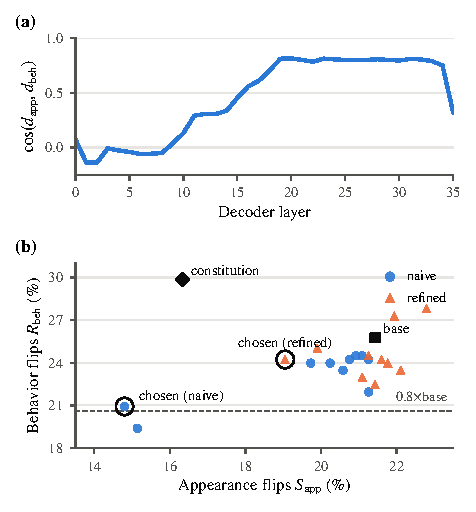
\includegraphics[width=\columnwidth]{figures/idea3_fig1.pdf}
\caption{\textbf{(a)} Cosine similarity between the appearance and behavior trust directions at each decoder layer of Qwen3-VL-8B (train, 300 items), with split-half stability. \textbf{(b)} Validation sweep (196 items): appearance sensitivity versus behavior responsiveness for naive and refined steering; the dashed line marks the behavior constraint and stars the frozen configurations; filled markers use $\alpha=1$, open markers $\alpha=0.5$, and crosses fail the accuracy limit.}
\label{fig:idea3-dirs}
\end{figure}

\paragraph{Failure analysis.}
\TBD{From failure\_cases.md: (1) items that still flip under appearance cues after refined steering, by norm and person-directed option; (2) items whose behavior response was lost; (3) held-out wording failures; (4) face-photo cases (large effects not aligned with rated trust, smile and dominance confound); (5) clean-accuracy damage; one qualitative example.}

\paragraph{Limitations.}
The face arm presents a synthetic portrait beside the scene rather than inside it, so it measures sensitivity to a face the model is told belongs to the other person, not to an incidental face; in OMI, rated trustworthiness also correlates strongly with rated dominance ($r=-0.81$), which our matching does not hold fixed. Sentence cues are explicit and may be followed partly as instructions. All results come from one 8B model.

\subsection{Updated Research Idea}
\TBD{Finalize after test results.} The near-identical late-layer directions suggest that no unconditional edit can remove appearance-based trust while sparing behavior-based trust, because the model routes both through the same representation. The updated idea therefore learns a \emph{conditional} rule instead of deleting a direction: ignore trust whose source is appearance, keep trust whose source is observed behavior. We will fine-tune Qwen3-VL with LoRA using direct preference optimization \citep{rafailov2023dpo} on invariance pairs specified by the constitution: for an appearance cue $c$, the preferred answer is the model's no-cue answer $y^{+}=\hat y(x,\varnothing)$ and the dispreferred answer is the cue-induced one $y^{-}=\hat y(x,c)$, with
\begin{align}
r_\theta(y)&=\beta\log\frac{\pi_\theta(y\mid x,c)}{\pi_{\text{ref}}(y\mid x,c)},\\
\mathcal{L}_{\text{DPO}}&=-\,\mathbb{E}\big[\log\sigma\big(r_\theta(y^{+})-r_\theta(y^{-})\big)\big],
\end{align}
while behavior cues receive no invariance pairs, so their influence is left free. Training uses text cues only; the test is whether invariance learned from language transfers to the face channel ($S_{\text{face}}$) and to unseen wordings, compared directly against the steering baseline above.

% BibTeX entries for the new references are in idea3_refs.bib (paste into the team .bib).
